%%%%%%%%%%%%%%%%%%%%%%%%%%%%%%%%%%%%%%%%%%%%%%%%%%%%%%%%%%%%%%%%%%%%%%%%%%%%%%
\chapter{Signal Processing Theory}
\label{cha:TheThesis}

%%%%%%%%%%%%%%%%%%%%%%%%%%%%%%%%%%%%%%%%%%%%%%%%%%%%%%%%%%%%%%%%%%%%%%%%%%%%%%
\section{Modulation from Baseband to RF}

%%%%%%%%%%%%%%%%%%%%%%%%%%%%%%%%%%%%%%%%%%%%%%%%%%%%%%%%%%%%%%%%%%%%%%%%%%%%%%
\section{Modulation from RF to Baseband}

%%%%%%%%%%%%%%%%%%%%%%%%%%%%%%%%%%%%%%%%%%%%%%%%%%%%%%%%%%%%%%%%%%%%%%%%%%%%%%
\section{Oversampling / Sample Rate Reduction}
%TODO: explain DSP functions that are actually used in Matlab FM demod
Example: \\
In case the multiplex signal needs to be stored in a file with 44.1 kHz samplerate, in order to avoid aliasing, a lowpass with a cutoff frequency of 15 kHz and sufficient attenutation before 19 kHz needs to be inserted before the decimation and file output.

%%%%%%%%%%%%%%%%%%%%%%%%%%%%%%%%%%%%%%%%%%%%%%%%%%%%%%%%%%%%%%%%%%%%%%%%%%%%%%
\section{Frequency Modulation in Broadcasting}
  %see literature/Present\_lec6\_AM\_FM.pdf\\
  %see lectures out of HSD/ESD

Frequency modulation (FM) is a widely used standard to transmit data streams.
The probably best known usecase therefor is commercial broadcast radio, where an audio stream is transmitted.
Devices to receive these streams are available for low prices to the public.

This chaper describes the main properties of broadcast FM, such as the mathematical description, frequency bands that are used, or the specific frequency parts within a channel spectrum.

%%%%%%%%%%%%%%%%%%%%%%%%%%%%%%%%%%%%%%%%%%%%%%%%%%%%%%%%%%%%%%%%%%%%%%%%%%%%%%
\subsection{Mathematical description}

The mathematical description of an FM baseband signal can be described with the formulas presented in this section.
FM encodes the information content in its instantanious frequency.
This means that the measured frequency at any moment in time represents a specific value of a transmitted message.
For a general classification, FM belongs to the group of angle, or phase modulated signals (PM).
The simple reason therefor is, that a frequency has a direct relationship to an angle, if the signal is seen on a unit circle.\\

The instantanious frequency $f_i$ of an FM signal can be described as
\begin{equation}
  f_i = f_c + \Delta f \cdot m(t)
\end{equation}
where $f_c$ is the carrier- or center frequency, $\Delta f$ is the maximum frequency deviation and $m(t)$ is the information or message signal that is to be transmitted.
Simply looking at this equation, the frequency deviation, which is sometimes also called the swing, varies in the range between $f_c \pm \Delta f$.

Considering the relationship between frequency and angle, as described above, and after some simple substitutions which will not be described into detail here, the equation for a generic frequency modulated wave is the following
\begin{equation}
  s(t) = A_c\ cos \Big( 2 \pi f_c t + 2 \pi k_f \int m(t) dt \Big)
  \label{equ:fm_func}
\end{equation}
where $A_c$ is the amplitude of the resulting FM signal and $k_f$ is the frequency sensitivity factor.
This sensitivity factor has a direct relationship with the modulation index $\beta$.
\begin{equation}
  \beta = \frac{\Delta f}{f_m} = \frac{k_f A_m}{f_m}
\end{equation}
where $f_m$ is the highest existing frequency, or the bandwidth of the information signal.
% More info on modulation index: https://fas.org/man/dod-101/navy/docs/es310/FM.htm

Formula \eqref{equ:fm_func} describes a frequency modulated signal with a generic message signal $m(t)$.
A widely used example application of FM is broadcast radio, where audio streams are transmitted.
An audio stream can be described as a cosine wave.
Therefore, the information signal that is to be transmitted in broadcast radio can be represented as a cosine wave in the form of
\begin{equation}
  m(t) = A_m\ cos(2 \pi f_m t).
\end{equation}
By inserting this message signal into the generic FM formula \eqref{equ:fm_func}, the final equation for an FM signal transforms into the following form.
\begin{equation}
  y(t) = A_c\ cos \Big(2 \pi f_c t + \beta\ sin(2 \pi f_m t)\Big )
\end{equation}
Several formulas, as well as their derivations are described according to \cite{ref_FM_Maths_Info_1}\cite{ref_FMMaths2}.

%%%%%%%%%%%%%%%%%%%%%%%%%%%%%%%%%%%%%%%%%%%%%%%%%%%%%%%%%%%%%%%%%%%%%%%%%%%%%%
\subsection{Frequency Band}

The frequency band that is used for FM broadcasting is defined worldwide and spans from 87.5 to 108 MHz.
However, some countries only partially use the band \cite{ref_itu_regulations}.
The range is located within the so-called Very-High-Frequency (VHF) band, which is open to the public in terms of usage.
This means, that any transmitter may use the specified frequency range freely.
Austria allowed the legal usage in 2006 \cite{ref_austria_rundfunkgesetz_2006}.
However, the transmission power needs to be limited, so that neighboring receivers are not disturbed in receiving any existing channels.
The European Commision specifies the power limit as 50 nW of effective radiated power (ERP) \cite{ref_eu_commision_radio_spectrum}.
Another limitation is, that a transmitter must be capable to transmit on multiple center frequencies within the broadcasting band.
It must not be fixed to a single center frequency.
Through this specification, a transmitter is capable of switching its transmission center frequency, in order to avoid interference with another transmitters signal.

In a practical usecase this means that a transmitter needs to select a channel or frequency range, that is not already occupied by an official transmitter.
If a free range is found, the transmitter may start sending an FM signal with the mentioned power limitations \cite{ref_ebu_fm_modulators_in_europe_power_regulations}.

%https://www.ris.bka.gv.at/GeltendeFassung.wxe?Abfrage=Bundesnormen&Gesetzesnummer=20008807


%%%%%%%%%%%%%%%%%%%%%%%%%%%%%%%%%%%%%%%%%%%%%%%%%%%%%%%%%%%%%%%%%%%%%%%%%%%%%%
\subsection{Frequency Spectrum of a Broadcast FM Channel}

The entire FM broadcasting band from 87.5 to 108 MHz divides into multiple channels which can be used.
In Europe, the European Telecommunications Standards Institute (ETSI) sets the respective standards for the usage of these frequencies.
The main specifications for a single FM broadcasting channel are explained in this section.\\

Each channel may allocate a bandwidth of 200 kHz.
Within one of these channels, the maximum deviation from the center frequency shall not exceed 75 kHz.
This leaves a guard band of 25 kHz on either side, to minimize interference with adjacent channels.
Center frequencies may be allocated on multiples of 100 kHz.
However, neighboring channels need to be considered therefore, since this may result in an overlap in the spectrum.\\

Fig.\ref{fig_channel_baseband_freqs} shows the frequency spectrum of a single channel, located at its carrier- or center frequency.
For a better overview, only the positive spectum part is shown.
The negative part is an exact mirror, because the transmitted and received signals from the antenna are real signals - they do not have an imaginary part.
The spectrum consists of multiple parts. Therefore, it is also referred to as `multiplex signal' in the literature. Several parts are described in the following paragraphs.

\begin{figure}[!h]
  \centering
    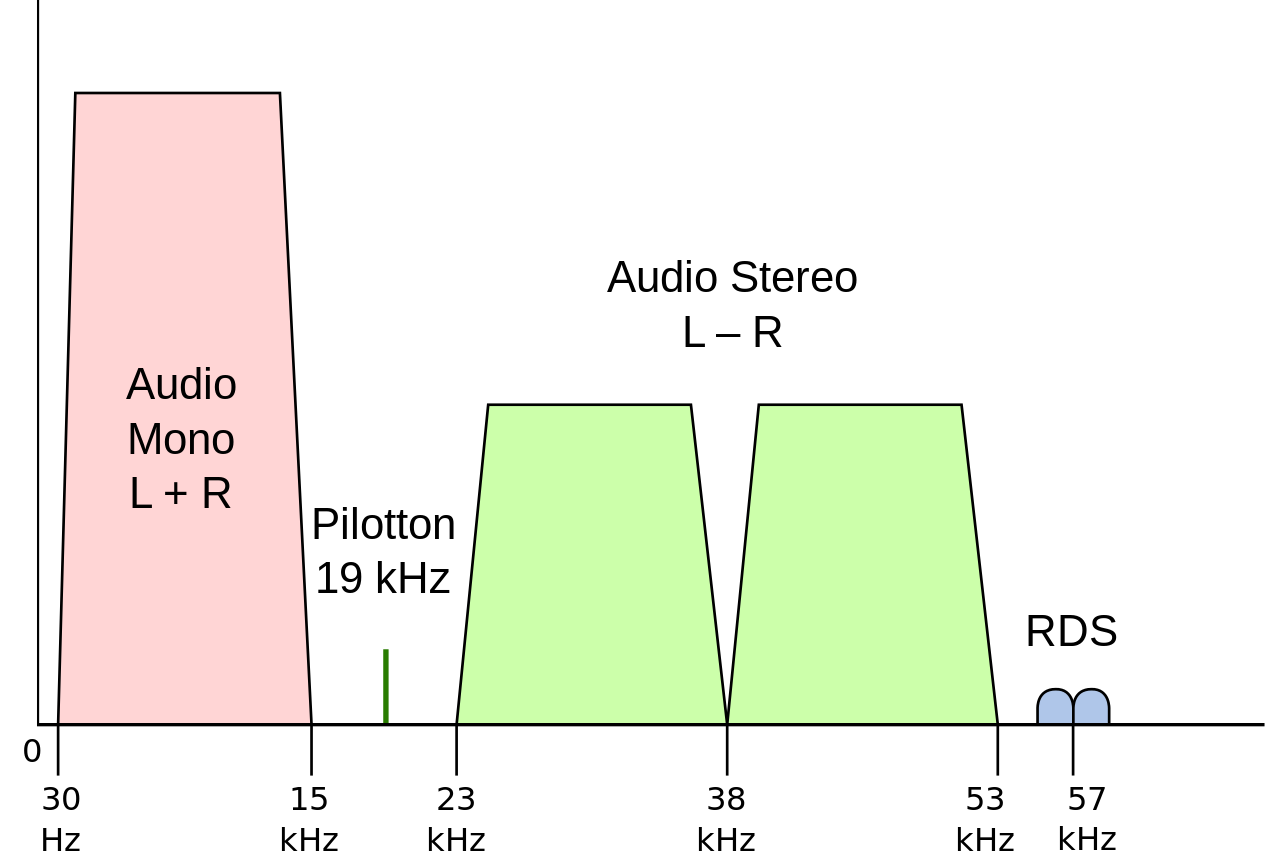
\includegraphics[width=9cm]{img/fm-channel-baseband.png}
  \caption{Allocation of frequencies in an FM channel \cite{ref_fig_channel_freqs}.}
  \label{fig_channel_baseband_freqs}
\end{figure}

%%%%%%%%%%%%%%%%%%%%%%%%%%%%%%%%%%%%%%%%%%%%%%%%%%%%%%%%%%%%%%%%%%%%%%%%%%%%%%
\subsubsection{Mono Audio Part}

The mono audio stream is located between 30 Hz and 15 kHz.
This signal is built by the sum of the left and right audio channels.
%The lower limit at 30 Hz is to prevent the transmission of a direct current (DC) part, which would require a large amount of power in transmission.
%This effect is one of the downsides of amplitude modulation (AM), where the carrier is located at the channels' center frequeny and requires a high transmission power. % TODO: check this fact
The upper limit at 15 kHz is chosen to maintain a sufficient spacing to the first subcarrier.

For audio streaming, as in FM broadcasting, this is not a limitation, since it is unlikely to have frequencies higher than 15 kHz in an audio stream.
Also, this already reaches the upper limit of the human ears' bandwith, so higher spectral parts will not be heard anyway.

%%%%%%%%%%%%%%%%%%%%%%%%%%%%%%%%%%%%%%%%%%%%%%%%%%%%%%%%%%%%%%%%%%%%%%%%%%%%%%
\subsubsection{Pilot Tone}

The first subcarrier is allocated at an offset of 19 kHz from the center frequency.
This subcarrier is also called the 'pilot tone', since it is a continuous signal.
It is independent of any varying message signal content.
The pilot tone is used for stereo audio demodulation.
To regenerate a stereo audio signal, the left and right audio channels need to be recovered correctly.

%%%%%%%%%%%%%%%%%%%%%%%%%%%%%%%%%%%%%%%%%%%%%%%%%%%%%%%%%%%%%%%%%%%%%%%%%%%%%%
\subsubsection{Stereo Audio Difference}

A signal that is constructed by the difference between the left and right audio channel is modulated on a 38 kHz subcarrier.
This subcarrier is an integer multiple of the pilot tone at 19 kHz, for practical reasons.
However, the 38 kHz carrier is suppressed and thus not visible in the received spectrum.
The modulation technique that is used for this spectral part is called dual-sideband suppressed-carrier (DSB-SC).
Even though the carrier is suppressed, it can still be recovered, because it is phase coherent with the 19 kHz pilot tone per definition.

The bandwidth for this difference-signal spans 15 kHz on either side of the subcarrier.
It is used to generate a stereo audio signal, in combination with the mono signal.
This process is explained into more detail in chapter \ref{sec_fm_sig_demod}.

%%%%%%%%%%%%%%%%%%%%%%%%%%%%%%%%%%%%%%%%%%%%%%%%%%%%%%%%%%%%%%%%%%%%%%%%%%%%%%
\subsubsection{Additional Services}

Considering all these parts in the spectrum, there is still free bandwidth available to use up to the maximum channel bandwitdh of 100 kHz in one sideband.
Because of that, additional services were added to the pure audio transmission, to provide additional data services and information.

Services that were implemented are the Data Radio Channel (DARC), which is mostly used in Japan and the USA, the Subsidary Communication Authorization (SCA) and the Radio Data System (RDS) \cite{ref_rohde_u_schwarz}.
Out of these, RDS is the most significant service in Europe.
It is used to transmit additional information about the channel, such as the radio stations' name, the currently playing songs' title or traffic information.\\

\noindent
The information about the frequency spectrum was taken from \cite{ref_fm_broadcast_tutorial_and_basics}.

%%%%%%%%%%%%%%%%%%%%%%%%%%%%%%%%%%%%%%%%%%%%%%%%%%%%%%%%%%%%%%%%%%%%%%%%%%%%%%
\section{Algorithms for Digital FM Demodulation}
\label{sec:algorithms-for-digital-fm-demodulation}
  %see literature/FmDemodulator.pdf (Sect. 3.3)
  %see literature/00476180 Digital FM Demodulator for FM, TV, and Wireless.pdf (Sect. II and III)

An FM signal that is received, for example from an antenna, needs to be demodulated in order to decode its actual data content.
In general, an FM demodulator serves the purpose to transform a frequency modulated signal (FM) into an amplitude modulated signal (AM), so that AM signal processing techniques can be applied afterwards.\\

The radio frequency antenna signal usually needs to be amplified, bandpass-filtered, and down-converted to baseband, using subsampling and quadrature-mixing, or similar strategies.
This part of the signal processing chain is assumed to be working correctly and is out of the scope of this chapter. %TODO: write up/down conversion in other chapter?
The FM signal that is evaluated here is assumed to be a quadrature-mixed signal in baseband, which means that inphase and quadrature (I/Q) signals are available.

%TODO: show downconversion path (maybe as a figure?)
%https://www.veron.nl/wp-content/uploads/2014/01/FmDemodulator.pdf

In the following sections, two digital FM demodulator variants are described.

% TODO: add img/discrimination_method_bd2.png here (?)

%%%%%%%%%%%%%%%%%%%%%%%%%%%%%%%%%%%%%%%%%%%%%%%%%%%%%%%%%%%%%%%%%%%%%%%%%%%%%%
\subsection{Frequency Discriminator}

A frequency discriminator generates an output that is directly proportional to the frequency of the input FM signal.
In other words, it converts FM to AM.
The discriminator consists of two main parts - a differentiator and an envelope detector.
Different strategies can be implemented for both parts.
A block diagram for a frequency discriminator with its two main parts is shown in Fig.\ref{fig:bd_freq_discriminator}.

\includepicture [0.7] [0] {Frequency discriminator block diagram \cite{ref_fig_freq_discriminator}.} {bd_freq_discriminator} {img/bd_freq_discriminator}

%%%%%%%%%%%%%%%%%%%%%%%%%%%%%%%%%%%%%%%%%%%%%%%%%%%%%%%%%%%%%%%%%%%%%%%%%%%%%%
\subsubsection{Differentiator}

The differentiator already converts the FM signal into an AM signal, but still leaves an FM content.
The transformation that happens here can be expressed in a formula, by simply differentiating Eq.\eqref{equ:fm_func}.
This operation, with some additional simple algebraic transformations, results in
\begin{equation}
  \frac{d s(t)}{dt} = A_c 2 \pi \Big[f_c + k_f m(t) \Big] sin \Big(\omega_c t + 2 \pi k_f \int m(t) dt -pi \Big)
  \label{equ:fm_demod_discriminator}
\end{equation}

This formula shows the AM and an FM contents clearly.
The FM part is described by the sine function, with its argument.
The more important part is the AM part, which resembles the message signal.
It is described by the term within the square brackets.

A time-domain example for this signal is shown in the top left diagram in Fig.\ref{fig:time_domain_envelope_detect}.\\

An important requirement for the differentiator is, that the input signal is of a constant amplitude \cite{ref_schnyder_haller}.
The transmitted signal is subject to random additive noise on the transmission channel.
The differentiator would deliver wrong results because of this noise, when substracting two consecutive samples, as described in Eq.\eqref{equ:differentiator_two_samples}.
To achieve a constant amplitude, the received complex baseband signal $s(t)$ can be normalized to a value of one.
\begin{equation}
  s_{norm} = \frac{s}{|s|} = \frac{A(n)\ e^{j\phi_{FM}(n)}}{|{A(n)\ e^{j\phi_{FM}(n)}|}} = e^{j\phi_{FM}(n)}
\end{equation}
\begin{equation}
  e^{j\phi_{FM}(n)} = |1|
\end{equation}

In a hardware implementation, a differentiation is simply performed by substracting two consecutive samples, like
\begin{equation}
  \frac{d s(t)}{dt} = s(t) - s(t-\Delta t)
  \label{equ:differentiator_two_samples}
\end{equation}
where $\Delta t$ is the inverse of the sample frequency.\\ %TODO: check this (i'm using a 3-tap FIR in FPGA)

%%%%%%%%%%%%%%%%%%%%%%%%%%%%%%%%%%%%%%%%%%%%%%%%%%%%%%%%%%%%%%%%%%%%%%%%%%%%%%
\subsubsection{Envelope Detector}

The differentiated signal still consists of a FM part, as explained above, using Eq.\eqref{equ:fm_demod_discriminator}.
In order to remove this high-frequeny part and extract the low-frequency envelope, the signal needs to be fed into an envelope detector.
A block diagram is shown in Fig.\ref{fig:bd_freq_discriminator}.

The method implemented in Fig.\ref{fig:time_domain_envelope_detect} is one of the most simple ones and is usually referred to as `Asynchronous Half-Wave Envelope Detector'\cite{ref_envelope_detector}.
It consists of a thresholding unit to remove negative values and a conventional lowpass filter.
In analog implementations, the thresholding unit is a diode.
The cutoff frequency of the lowpass needs to be adapted to the envelope signals' maximum frequency.
It needs to be able to follow the signal, but also sufficiently smooth out the rectified signal.\\

Different methods may be implemented for the envelope detector.
For example, an `Asynchronous Full-Wave Envelope Detector' can be used.
Therefor, the previous method only needs to swap the thresholding unit with an unit that calculates the absolut value.
In that architecture, a full-wave rectification is performed on the signal, which significantly improves the envelope detection accuracy \cite{ref_envelope_detector}.
The envelope is followed more exactly, because of the higher power that is available in the signal, since the entire signal is taken into account, and not only the positive half, as in the previous half-wave method.

\includepicture [0.75] [0] {Time-domain signals in envelope detection \cite{ref_roppel}.} {time_domain_envelope_detect} {img/envelope-detect-time-domain.jpg}

%%%%%%%%%%%%%%%%%%%%%%%%%%%%%%%%%%%%%%%%%%%%%%%%%%%%%%%%%%%%%%%%%%%%%%%%%%%%%%
\subsection{Phase-Locked Loop}
%%%%%%%%%%%%%%%%%%%%%%%%%%%%%%%%%%%%%%%%%%%%%%%%%%%%%%%%%%%%%%%%%%%%%%%%%%%%%%
%\subsubsection{Baseband Delay Demodulator}
%%%%%%%%%%%%%%%%%%%%%%%%%%%%%%%%%%%%%%%%%%%%%%%%%%%%%%%%%%%%%%%%%%%%%%%%%%%%%%
%\subsubsection{Phase-Adapter Demodulator}
%%%%%%%%%%%%%%%%%%%%%%%%%%%%%%%%%%%%%%%%%%%%%%%%%%%%%%%%%%%%%%%%%%%%%%%%%%%%%%
%\subsubsection{Mixed Demodulator}

%TODO: explain a PLL in some more detail (block diagram)
A Phase-Locked Loop (PLL) can also be used to transform an FM signal to an AM signal.
A PLL is a feedback loop that is usually used to generate an output signal that has a fixed phase reference to its input.
In the case of FM demodulation, the loop filter in the feedback branch is configured to be able to follow the frequency variations on the input, which is directly related to the encoded information.
The output of the PLL directly delivers an AM signal, which corresponds to the transmitted information. \cite{ref_schnyder_haller}

FM demodulation with a PLL is not described into more detail, since this thesis is focussing on the concept of an entire system architecture.

%%%%%%%%%%%%%%%%%%%%%%%%%%%%%%%%%%%%%%%%%%%%%%%%%%%%%%%%%%%%%%%%%%%%%%%%%%%%%%
\section{Demodulation of Broadcast FM}

This chapter describes the demodulation of the information content of an FM broadcast channel, as it is used in commercial FM radio broadcasting.
The assumption here is, that the actual FM demodulation, as described in chapter \ref{sec:algorithms-for-digital-fm-demodulation} is already done correctly.
A frequency spectrum of the multiplex signal of an FM channel is shown in Fig.\ref{fig_channel_baseband_freqs}.

%%%%%%%%%%%%%%%%%%%%%%%%%%%%%%%%%%%%%%%%%%%%%%%%%%%%%%%%%%%%%%%%%%%%%%%%%%%%%%
\subsection{Mono Audio}
\label{subsec:demod_mono}

The first part of the channel frequency spectrum is the mono audio signal.
It is the summation signal of the left and right audio channel.
Thus, it contains enough information to replay an audio stream in mono quality.
A mono receiver can thus simply replay the so-called multiplex signal that is produced by the FM demodulator, without any further filtering or processing.
The 19 kHz pilot tone, and any higher frequency components, will not be audible by most people, because it is outside of the range of a human ear.
Besides that, any used speaker may also be unable to produce a frequency in this range.\\

Consequently, in order to demodulate this spectral part, a lowpass filter is required.
The filter needs to have a cutoff frequency of 15 kHz, to allow the entire mono audio spectrum to pass.
Sufficient attenutation must be available before 19 kHz, in order to suppress the pilot tone.

%%%%%%%%%%%%%%%%%%%%%%%%%%%%%%%%%%%%%%%%%%%%%%%%%%%%%%%%%%%%%%%%%%%%%%%%%%%%%%
\subsection{Stereo Audio}

The demodulation of an FM channel to recover a stereo audio signal, requires a more sophisticated approach and multiple steps in signal processing.
Two parts need to be combined in order to achieve stereo.
The sum and the difference of the left and right audio channel signals - the mono and the stereo difference part, respectively.
The following equations need to be applied, to compute a left and a right channel.

\begin{equation}
  \begin{split}
    (L+R) + (L-R) = (2)L \\
    (L+R) - (L-R) = (2)R
    \label{equ_stereo_from_sum_diff}
  \end{split}
\end{equation}

where $(L+R)$ represents the mono part and $(L-R)$ the stereo difference.\\

The block diagram in Fig.\ref{fig_bd_stereo_demod} illustrates the signal processing chain for stereo audio.
In the block diagram, $x(t)$ represents the multiplex signal from the FM demodulator.
The signals $x_l(t)$ and $x_r(t)$ describe the left and right audio signal, respectively.\\

\begin{figure}[!h]
  \centering
    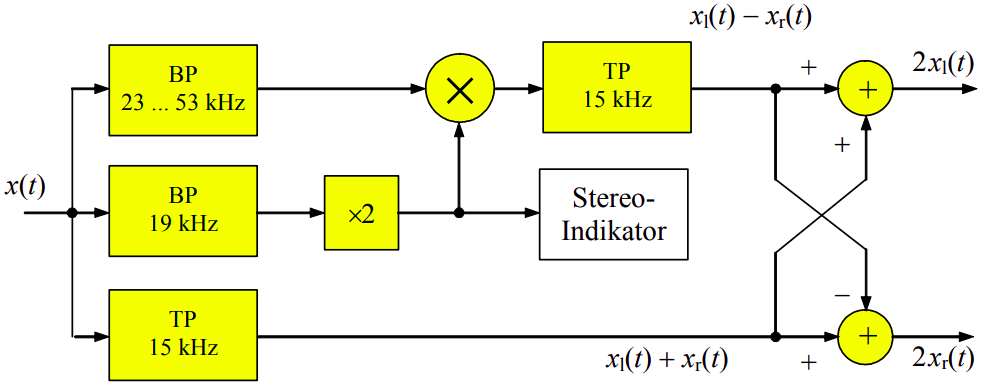
\includegraphics[width=8.8cm]{img/fm-demod-stereo-audio.png}
  \caption{Block diagram of FM stereo audio demodulation \cite{ref_roppel}.}
  \label{fig_bd_stereo_demod}
\end{figure}

The central branch selects the pilot tone at 19 kHz with a bandpass filter.
This bandpass needs to have a frequency response that is sharp enough to have a sufficient attenuation at $\pm$4 kHz, since this is where the mono and difference signals' frequency spectra are allocated.
Afterwards, the pilot tone frequency is doubled to achieve a 38 kHz subcarrier.
This guarantees a phase-coherency between pilot and subcarrier, which is required to correctly shift the difference signal down to baseband.

The frequency doubling can be implemented with multiple methods.
The pilot tone can be modulated by simply multiplying it with itself.
Another option is to use a PLL and configure it to generate the double frequency at its output.
The PLL lock indicator can then be re-used as an indicator, whether a pilot tone is existent.\\

In the upper branch, a bandpass filter selects the difference signal with ranges from 23 to 53 kHz.
It is then modulated to baseband by the previously generated 38 kHz subcarrier.
Subsequently, a lowpass limits signal bandwidth to 15 kHz, which removes the generated modulation artifacts.\\

The lower branch lowpass-filters the summation, or mono signal, as described in paragraph \ref{subsec:demod_mono}.\\

The rightmost part in the diagram performs the combination of the mono and the difference signal, according to Eq.\eqref{equ_stereo_from_sum_diff}.
